\chapter{Sezioni trasversali}

È possibile ottenere le sezioni trasversali del tracciato utilizzando il comando Corridors/Dynamic Section. È possibile visualizzare sulla sezione anche le aree e i relativi volumi di scavo e riporto.

\begin{figure}[H]
    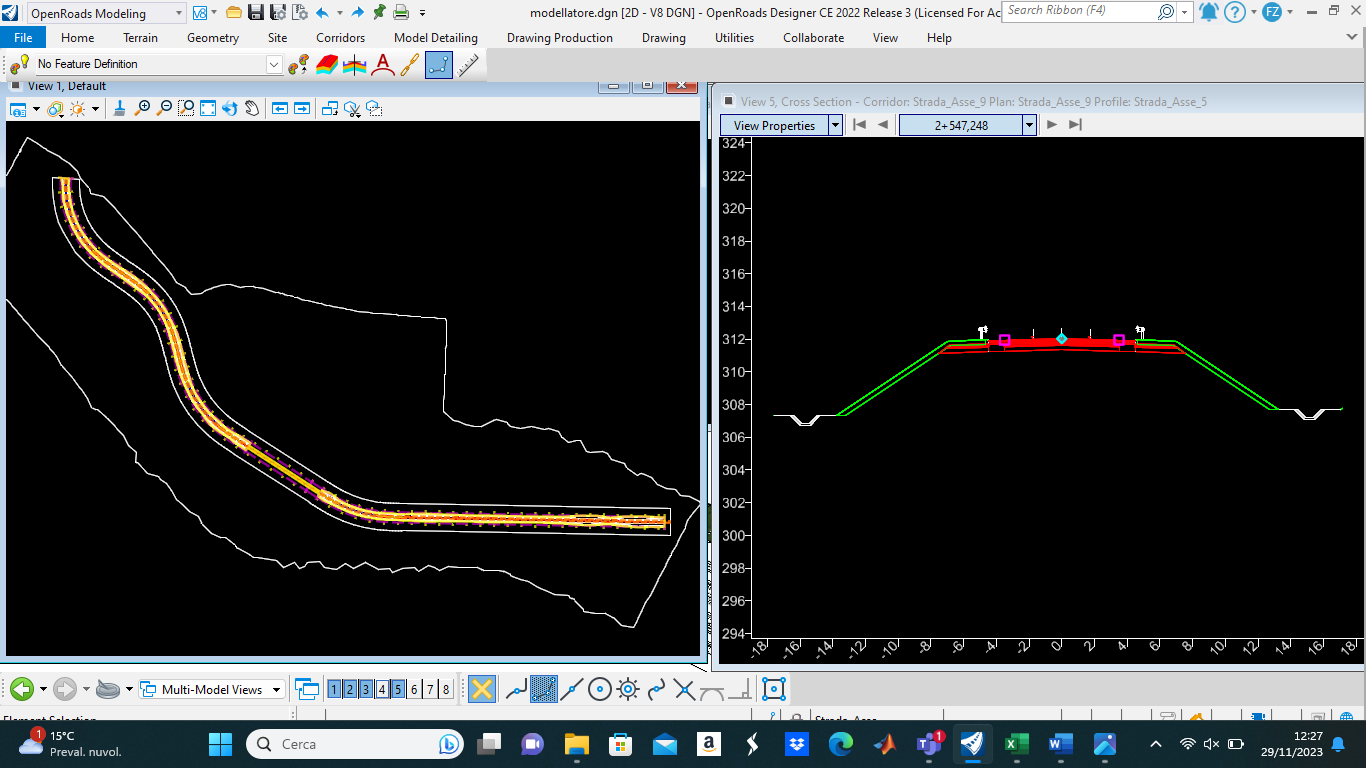
\includegraphics[width=\textwidth]{Figures/Sezione in rilevato.png}
      \caption{Sezione in rilevato}
      \label{Sezione in rilevato}
\end{figure}

\begin{figure}[H]
    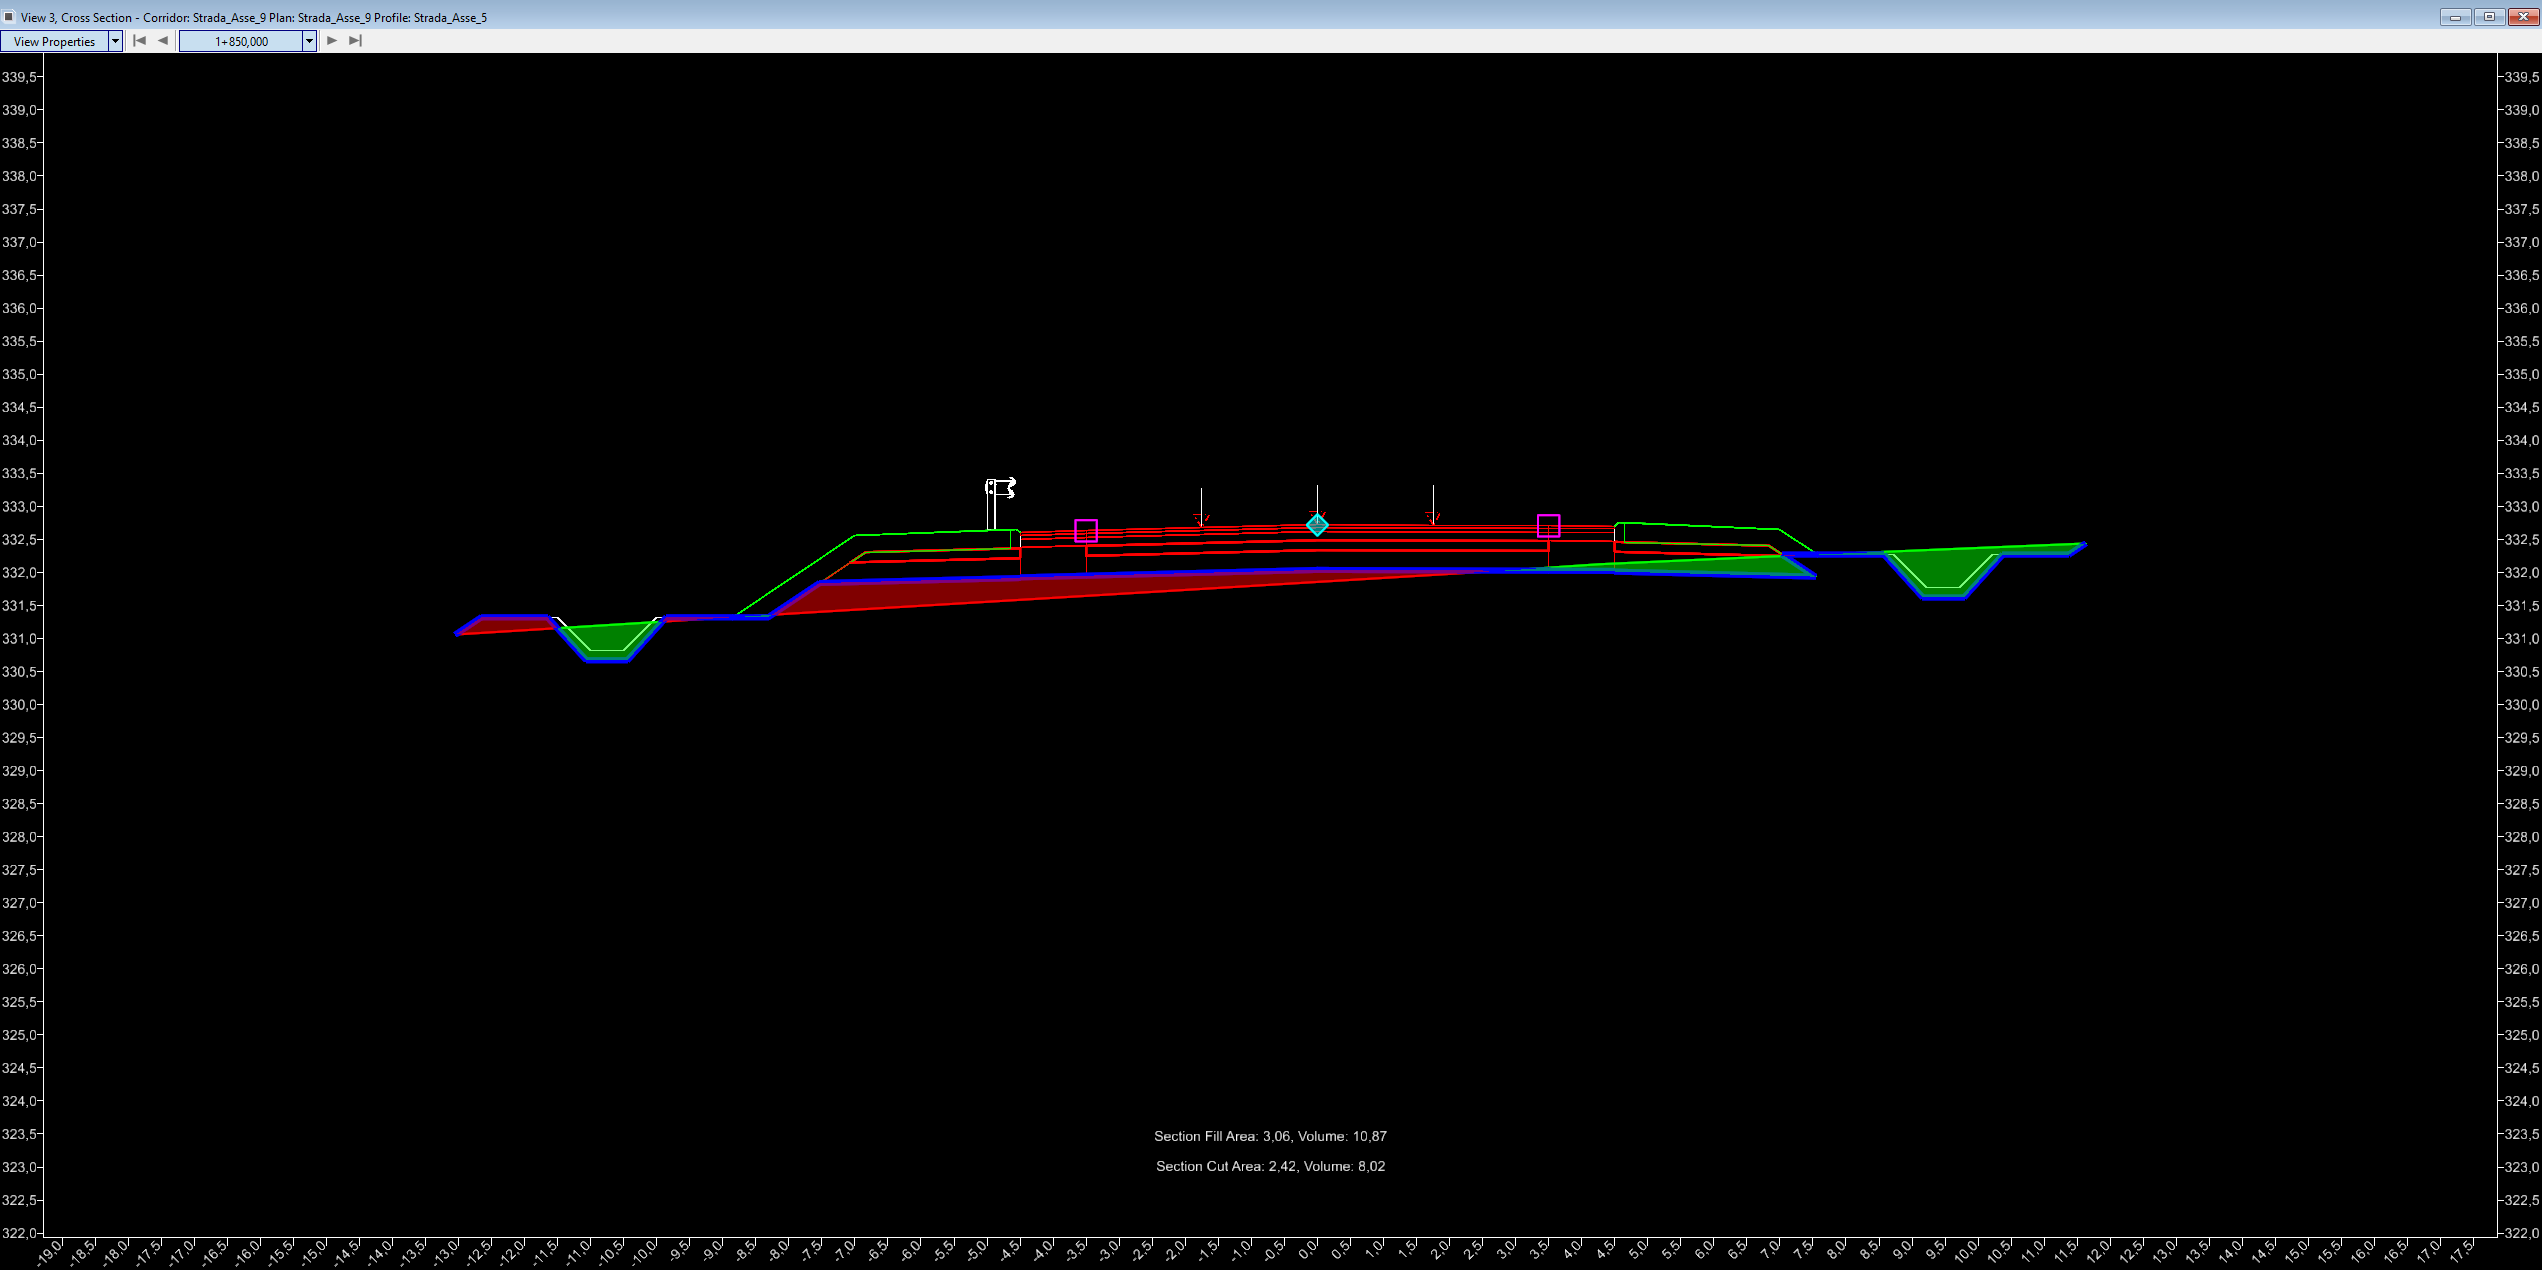
\includegraphics[width=\textwidth]{Figures/Sezione a mezzacosta.png}
      \caption{Sezione a mezzacosta}
      \label{Sezione a mezzacosta}
\end{figure}

\begin{figure}[H]
    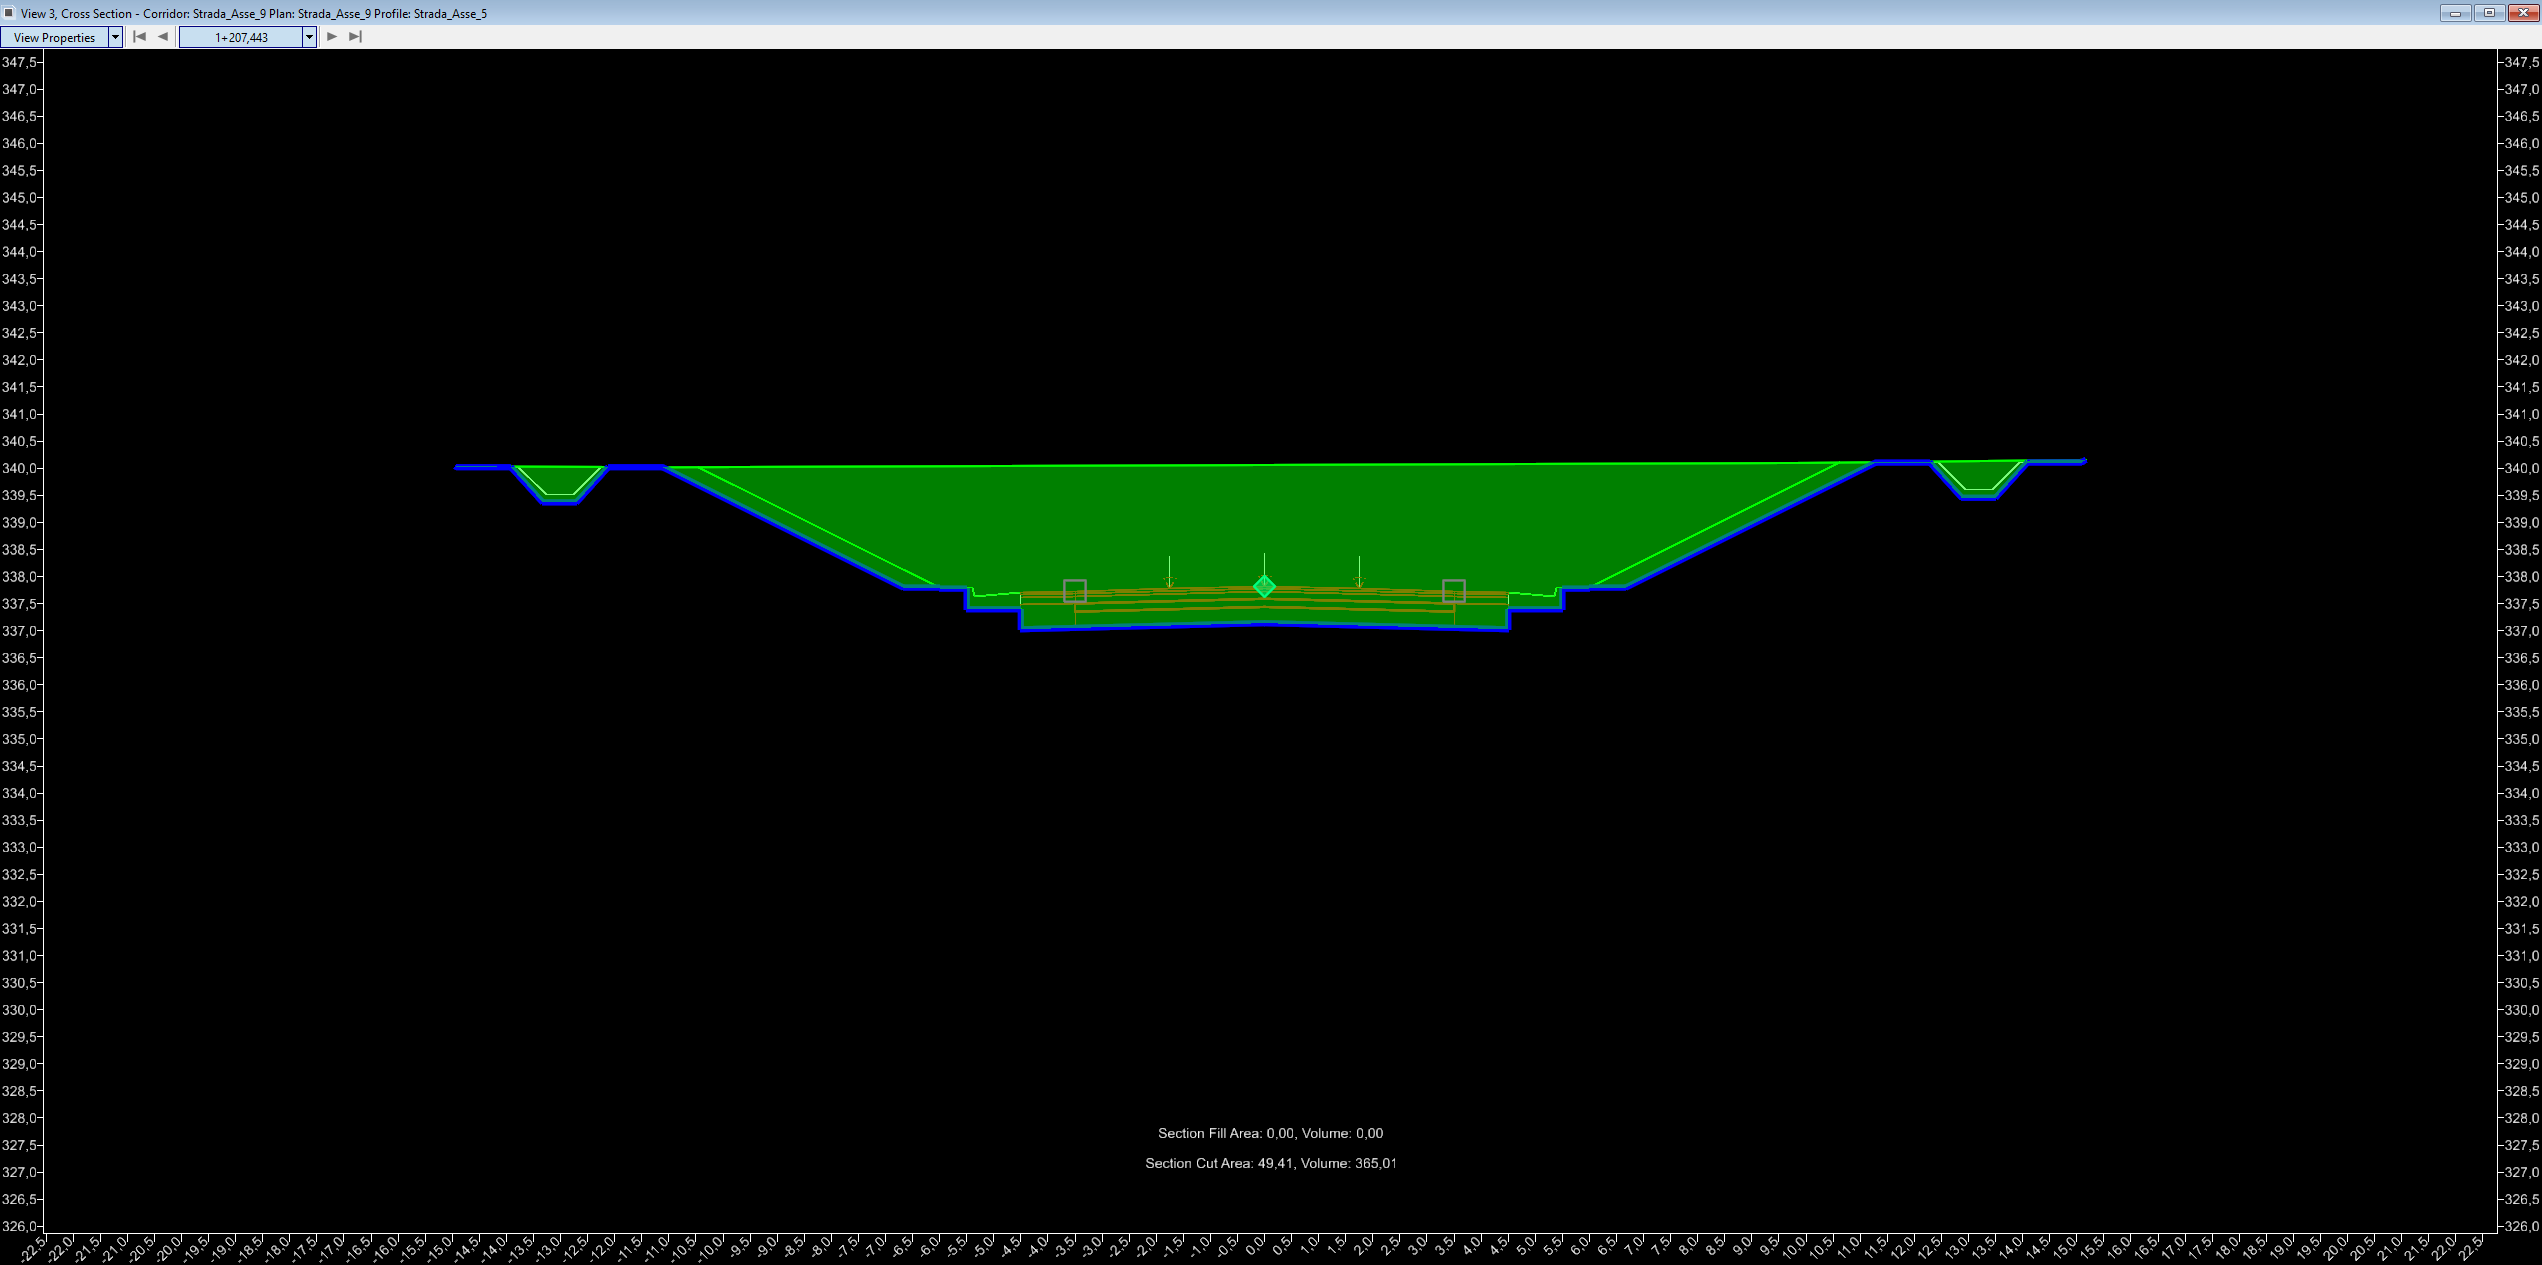
\includegraphics[width=\textwidth]{Figures/sezione in trincea.png}
      \caption{Sezione in trincea}
      \label{sezione in trincea}
\end{figure}

Attraverso il report del corridor è possibile, inoltre vedere quanto è il volume di scavo e di riporto complessivo o di ogni singola sezione (\ref{Corridorreport}).

\begin{figure}[H]
    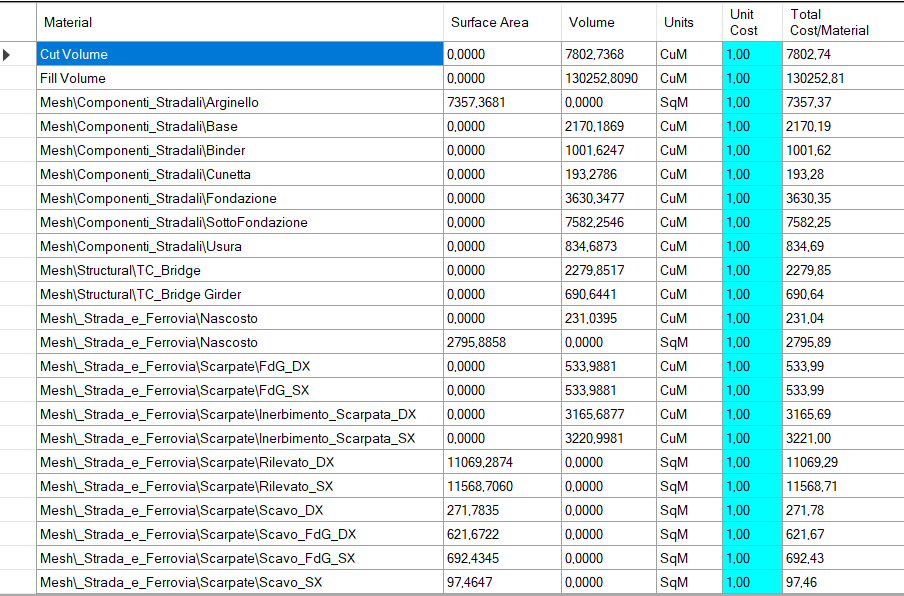
\includegraphics[width=\textwidth]{Figures/Corridor report.png}
      \caption{Corridor report}
      \label{Corridorreport}
\end{figure}

